%!TEX root=./pfc.tex
\chapter[Análisis de plataformas e-learning]{\label{}
Análisis de plataformas e-learning}

En este capítulo se va a realizar un análisis de las plataformas CMS (Course Management Systems) más utilizadas en la actualidad para seleccionar aquella que mejor se adapte a las necesidades de nuestro proyecto, indicando además los motivos de dicha selección. El análisis de las plataformas se realizará teniendo en cuenta las siguientes características:

\begin{itemize}
	\item \textbf{Requerimientos:} se tendrán en cuenta los requerimientos software y hardware, así como el tipo de licencia de la plataforma.
	\item \textbf{Seguridad:} debido a que se trata de una aplicación orientada a Internet es importante determinar la seguridad que ofrece.
	\item \textbf{Soporte:} en este apartado se analizará el tipo de soporte ofrecido por la plataforma, como pueden ser manuales, foros, etc.
	\item \textbf{Facilidad de uso:} al ser una plataforma orientada al aprendizaje, es decir, que va a ser constantemente accedida por profesores y alumnos que en la mayoría de los casos no serán expertos en e-learning, la facilidad de uso de la misma es un punto de vital importancia.
	\item \textbf{Funciones:} en este apartado se verán las funciones puramente informáticas de la plataforma, como pueden ser balanceo de carga, exportación del contenido de la base de datos, etc.
	\item \textbf{Administración:} la administración es uno de los puntos más importantes dentro de una plataforma. En este apartado se verán las capacidades de administración que tiene cada una.
	\item \textbf{Interoperatividad:} esta característica favorece el aprendizaje al fomentar la comunicación entre alumno-profesor y alumno-alumno. Por esta razón, se analizará y se valorará como punto favorable.
	\item \textbf{Aplicaciones soportadas:} además de la propia funcionalidad ofrecida por la plataforma, también se tendrá en cuenta la posibilidad de añadir aplicaciones extras dentro del entorno de la misma.
\end{itemize}

\section{Moodle}

\subsection{Introducción}

Moodle\cite{moodle} es una plataforma de aprendizaje a distancia basada en software libre, es decir, una aplicación diseñada para ayudar a los educadores a crear cursos de calidad en línea. Moodle fue creado por Martin Dougiamas, antiguo administrador de WebCT en la Universidad Curtin. Se basó en trabajos sobre el constructivismo en pedagogía, que afirman que el conocimiento se construye en la mente del estudiante en lugar de ser transmitido sin cambios a partir de libros o enseñanzas. Moodle ha ido evolucionando desde su creación en 1999 y actualmente se siguen desarrollando nuevas versiones cada vez con más frecuencia. En enero de 2005, la base de usuarios registrados incluye 2600 sitios en más de 100 países y está traducido a más de 50 idiomas.

\begin{figure}[h]
	\includegraphics[width=\textwidth]{./img/c2-moodle.eps}
	\caption{Plataforma e-learning Moodle}
\end{figure}

\subsection{Requerimientos}

\begin{itemize}
	\item Servidor de aplicación: PHP 4.1.2+. 
	\item Coste aproximado: Gratis.
	\item Base de datos: MySQL.
	\item Licencia: GNU GPL.
	\item Sistema operativo: Cualquiera. 
	\item Lenguaje de programación: PHP. 
	\item Servidor Web: Apache 1.3.
\end{itemize}

\subsection{Seguridad}

La seguridad en el sistema Moodle se limita a la autenticación de los usuarios mediante un servidor externo LDAP. También permite la autenticación de las cuentas creadas mediante servidores de correo o de news. Por otra parte, se permite la creación de distintos perfiles para mejorar el control de accesos a los recursos.

\subsection{Soporte}

En cuanto se refiere al soporte, es decir, lo que la organización que realiza el programa nos proporciona, tenemos que Moodle posee manuales comerciales en el mercado además de que proporciona una ayuda on-line, un foro público, una lista de correo y manuales para su utilización. Desde la web de Moodle se puede acceder a gran cantidad de documentación sobre la plataforma, así como, tener comunicación directa con desarrolladores experimentados para preguntar cualquier duda.

\subsection{Facilidad de uso}

Moodle tiene una gran facilidad de uso, permitiendo la inclusión de múltiples tipos de ficheros en los cursos, como pueden ser: test, libros digitales, ficheros HTML, ficheros PDF, hojas de cálculo EXCEL, ficheros WORD, etc. La asignación de profesores y estudiantes a los cursos, así como la creación y configuración de los mismos, no tiene ninguna complicación puesto que se realiza desde un simple menú. Posteriormente, la adición de recursos a los cursos se realiza de manera intuitiva sin ningún tipo de problema. Moodle tiene la posibilidad de cambiar su aspecto fácilmente gracias a las hojas de estilos (css).

\subsection{Funciones}

Moodle posee un sistema avanzado para cachear rápidamente contenidos de las páginas. Las plantillas para agilizar la navegación, además de permitir los duplicados de la base de datos para garantizar la seguridad. En su contra hay que destacar que permite balanceo de carga si hubiese varios servidores.

\subsection{Administración}

La administración de esta plataforma se puede dividir en administración de la plataforma, administración de usuarios y administración de cursos. La administración de la plataforma la realiza un administrador definido en la instalación de la misma. En este apartado se puede gestionar la interfaz del curso mediante la gestión de los temas y la gestión de los módulos incluidos en la plataforma. La administración de usuarios se basa en dos grandes grupos: estudiantes y profesores. Tanto unos como otros tienen un proceso de autenticación. El administrador es el encargado de asignar profesores a los cursos. Después de esto los profesores tienen control total del mismo. La administración de cursos se realiza por parte de los profesores y consiste en la creación de recursos del mismo de manera que los alumnos matriculados tengan acceso a los mismos.

\subsection{Interoperatividad}

Como herramientas de interoperatividad la plataforma Moodle posee las siguientes fundamentalmente:

\begin{itemize}
	\item Foros de discusión. Estos foros poseen las funciones normales de los mismos, edición de mensajes, adjuntar ficheros, etc.
	\item Chats. Permiten una interacción fluida mediante texto síncrono.
	\item Wikis. Permiten el desarrollo de wikis dentro de un curso.
	\item Talleres. Permite la subida de documentos así como la evaluación de los mismos entre iguales y la calificación por parte del profesor.
	\item Glosarios. Permite la realización de un listado de términos acerca de una temática concreta así como la evaluación de los mismos y la realización de comentarios por parte de otros alumnos y del profesor.
\end{itemize}

\subsection{Aplicaciones soportadas}

Una de las ventajas de esta plataforma es la posibilidad de incluir nuevos módulos. Esta característica combinada con la amplia expansión de la misma en todo el mundo dota a la plataforma de una gran capacidad de crecimiento mediante la inclusión de nuevos módulos desarrollados o mediante el desarrollo de un nuevo módulo en PHP que satisfaga las necesidades de los usuarios.

\section{WebCT}

\subsection{Introducción}

WebCT \cite{webct} comenzó como un proyecto del profesor Murray Golbert de la Universidad de Columbia para estudiar los efectos del aprendizaje online. WebCT se creó en 1997 como un producto comercial y es en 1999 cuando fue comprada por la Universal Learning Technology (UTL). Dentro de la plataforma WebCT se encuentran distintos productos de e-learning como pueden ser WebCT Vista y WebCT Campus Edition. A continuación se analizarán las características de WebCT Vista que se encuentra en el grupo de CMS más populares del momento.

\begin{figure}[h]
	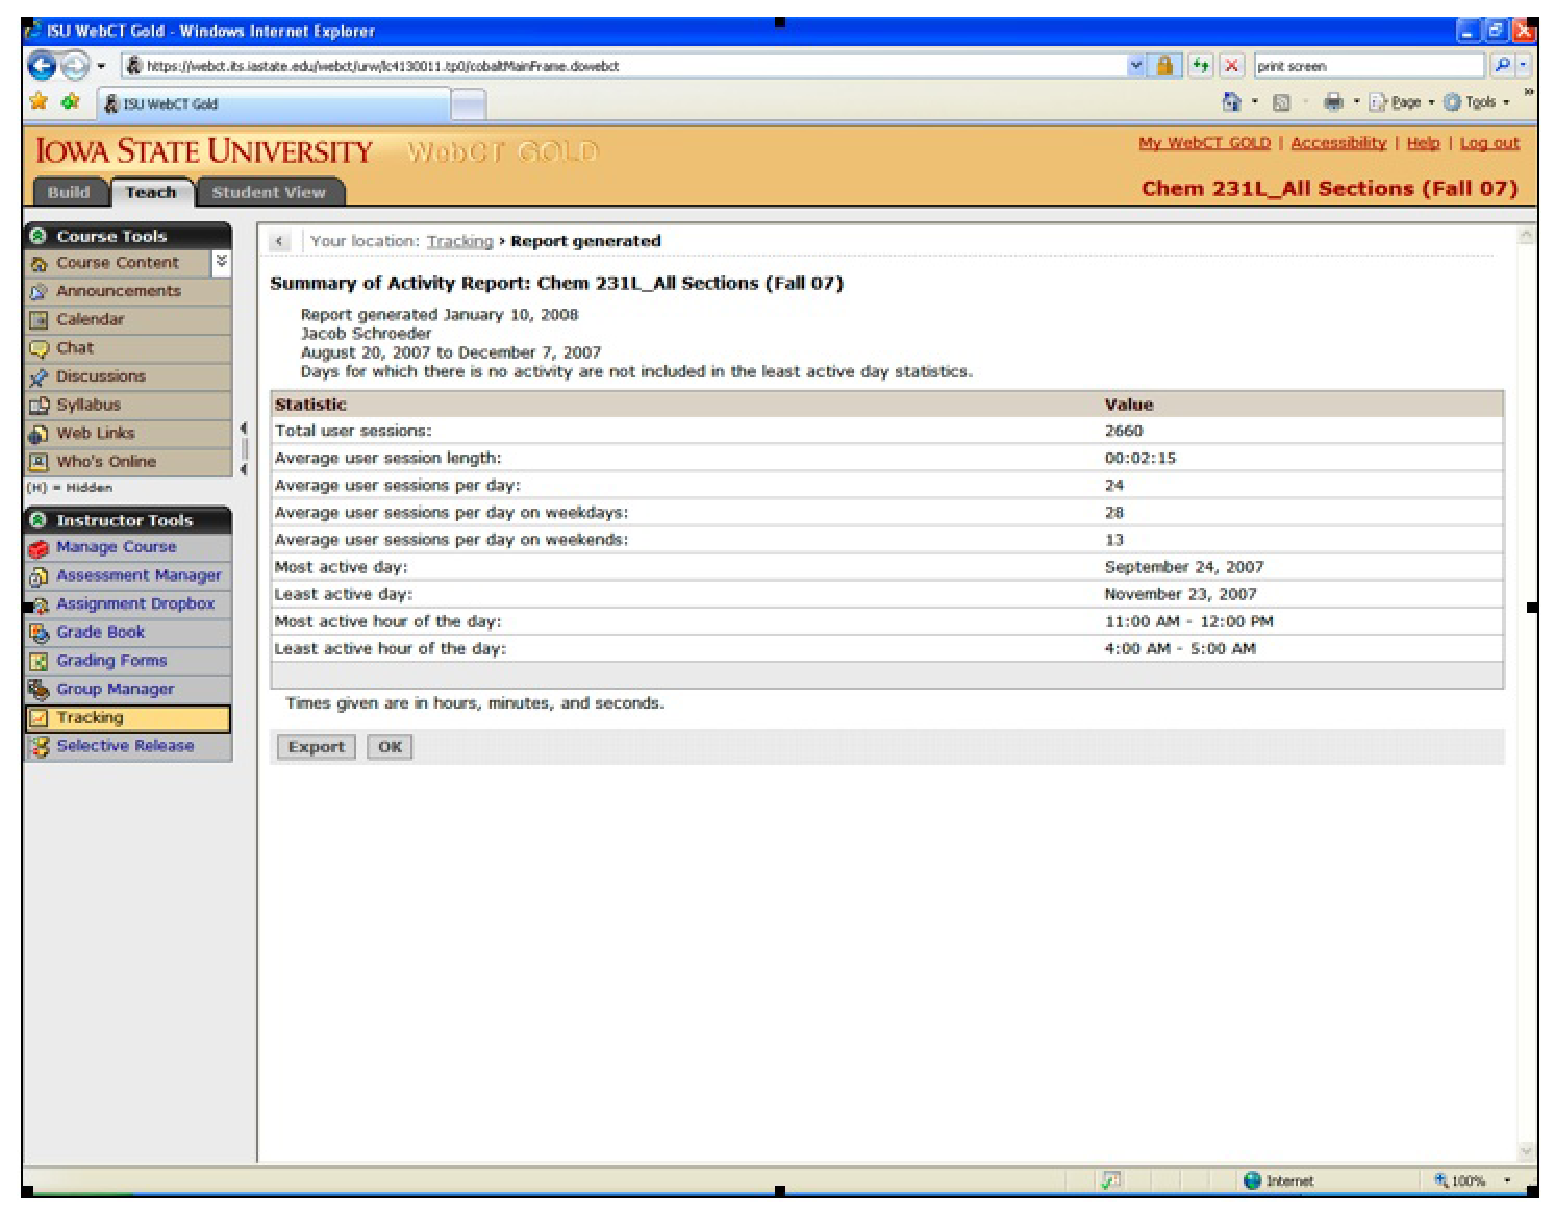
\includegraphics[width=\textwidth]{./img/c2-webct.eps}
	\caption{Plataforma e-learning WebCT}
\end{figure}

\subsection{Requerimientos}

\begin{itemize}
	\item Servidor de aplicaciones: La administración se realiza desde web. Los instaladores locales realizan la instalación de aplicaciones.
	\item Coste aproximado: La licencia de hasta 1000 usuarios para una organización sin ánimo de lucro es de aproximadamente 5000 €.
	\item Base de datos: Oracle 9i. Licencia: Anual por usuarios.
	\item Sistema operativo: RedHat Enterprise Linux, Sun SPARC Solaris 8 y 9, Windows 2000 Server SP 2 o Windows 2000 Advanced Server.
	\item Lenguaje de programación: Java y JavaScript. Servidor web: Apache.
\end{itemize}

\subsection{Seguridad}

Los administradores del sistema pueden proteger el acceso a los cursos mediante nombre de usuario y clave. Esta autenticación se realiza mediante un servidor LDAP externo o mediante el uso del protocolo Kerberos.

Se pueden establecer los parámetros de las claves, como longitud y cambios de la misma pasado un periodo de tiempo. Los logins de los usuarios pueden ser encriptados mediante el protocolo SSL.

Además de lo anteriormente comentado, el sistema WebCT esta completamente auditado, recogiendo registros de auditoría de todos los usuarios, así como guardando historial de accesos de los mismos.

\subsection{Soporte}

El soporte es uno de los puntos fuertes de WebCT debido a que se trata de una plataforma de pago. En este punto encontramos soporte para administradores, profesores y alumnos.

En cuanto al soporte para administradores se encuentran manuales on-line sobre administración, 'faqs' sobre administración y boletines de noticias, etc. Además de esto, encontramos soporte interactivo mediante listas de correo y foros de discusión. Por último se ofrece un área de descarga de software para administradores y un punto de contacto con el sistema de soporte de WebCT para solicitar ayuda en caso de que todo lo anterior no fuera suficiente.

El soporte ofrecido para profesores y alumnos del sistema es similar al ofrecido para los administradores, teniendo contenidos on-line, soporte interactivo y descarga de software.

\subsection{Facilidad de uso}

La creación de cursos esta basada en un editor web de uso fácil e intuitivo. La estructura básica y la navegación en los cursos no puede ser modificada, la ventaja que tiene este aspecto es que es de fácil aprendizaje para los novatos y el entorno se vuelve familiar para los alumnos avanzados. La desventaja que tiene es que se produce un proceso monótono al no poder adaptar la navegación a las necesidades del curso. El contenido de los cursos puede ser editado mediante un applet de Java que funciona como editor HTML. éste se utiliza para pequeñas modificaciones. Mientras que para modificaciones de mayor envergadura se usa el editor online instalado en el ordenador del administrador o profesor. En cuanto a la navegación de los cursos, decir que no se puede acceder a los contenidos mediante direcciones URL, posee un buen escalado de fuentes e imágenes y que los botones de retroceso y recarga en el navegador no funcionan como deberían. Al recargar una página se vuelve a la página inicial.

\subsection{Funciones}

En cuanto a las características que posee WebCT tenemos las siguientes: posee cacheado de páginas (lo cual mejora la navegación por los cursos), replicado de las bases de datos, trabajo bajo Oracle permitiendo así realizar copias de seguridad de manera rápida y fiable y, por último, balanceo de carga (que permite repartir el trabajo para evitar la saturación del sistema). Por el contrario, tiene la desventaja de que no existe la posibilidad de exportar el contenido del curso de manera estática para usarlo en un servidor local.

\subsection{Administración}

Las posibilidades de administración que posee WebCT permiten realizar la administración online del sitio web. Una característica especial es la actualización de los contenidos de manera temporal, es decir, se permite agregar o eliminar contenidos según períodos de tiempo. Otro punto importante en cuanto a la administración es la posibilidad de creación de perfiles para usuarios y la gestión de cada conjunto independientemente. En cuanto al registro de estudiantes para los cursos, se puede realizar directamente por medio del administrador o del profesor responsable del curso o bien, crear un proceso de registro automático para que los alumnos se matriculen en el propio curso.

\subsection{Interoperatividad}

Para fomentar el trabajo de los alumnos la plataforma WebCT posee diferentes herramientas que favorecen la interoperatividad, como son los foros de discusión, en los cuales los mensajes pueden contener ficheros adjuntos, ficheros HTML, etc. Otras características son el intercambio de ficheros mediante WebDAV o las listas de correo de los cursos, mediante las cuales se puede divulgar información. Por último posee un chat en tiempo real basado en Java y una pizarra compartida en la que se pueden compartir información con los alumnos. Esta pizarra permite escribir símbolos matemáticos así como subir imágenes y anotaciones.

\subsection{Aplicaciones soportadas}

WebCT posee gran cantidad de aplicaciones que dan soporte a los cursos generados como pueden ser Chats, foros, calendarios, estadísticas, etc. Un punto importante es que permite el trabajo en grupo (GroupWare), de manera que pueden generar grupos de manera aleatoria, generados por los profesores o bien grupos generados por los propios alumnos. Otra característica que posee WebCT es la posibilidad de que cada alumno se cree su propio portfolio en formato HTML, así como un espacio común para los alumnos, de manera que puedan intercambiar información y archivos.

\section{Ilias}

\subsection{Introducción}

La plataforma ILIAS \cite{ilias} fue desarrollada como parte del proyecto VIRTUS de la Universidad de Colonia. Es un sistema abierto usado por multitud de universidades debido a su licencia GNU. Este sistema está profundamente extendido y en los últimos tiempos está tomando importancia en multitud de universidades dentro de España. En Andalucía es el sistema que promueve la Junta de Andalucía como medio de enseñanza virtual. Como ejemplo está la Universidad de Jaén.

\begin{figure}[h]
	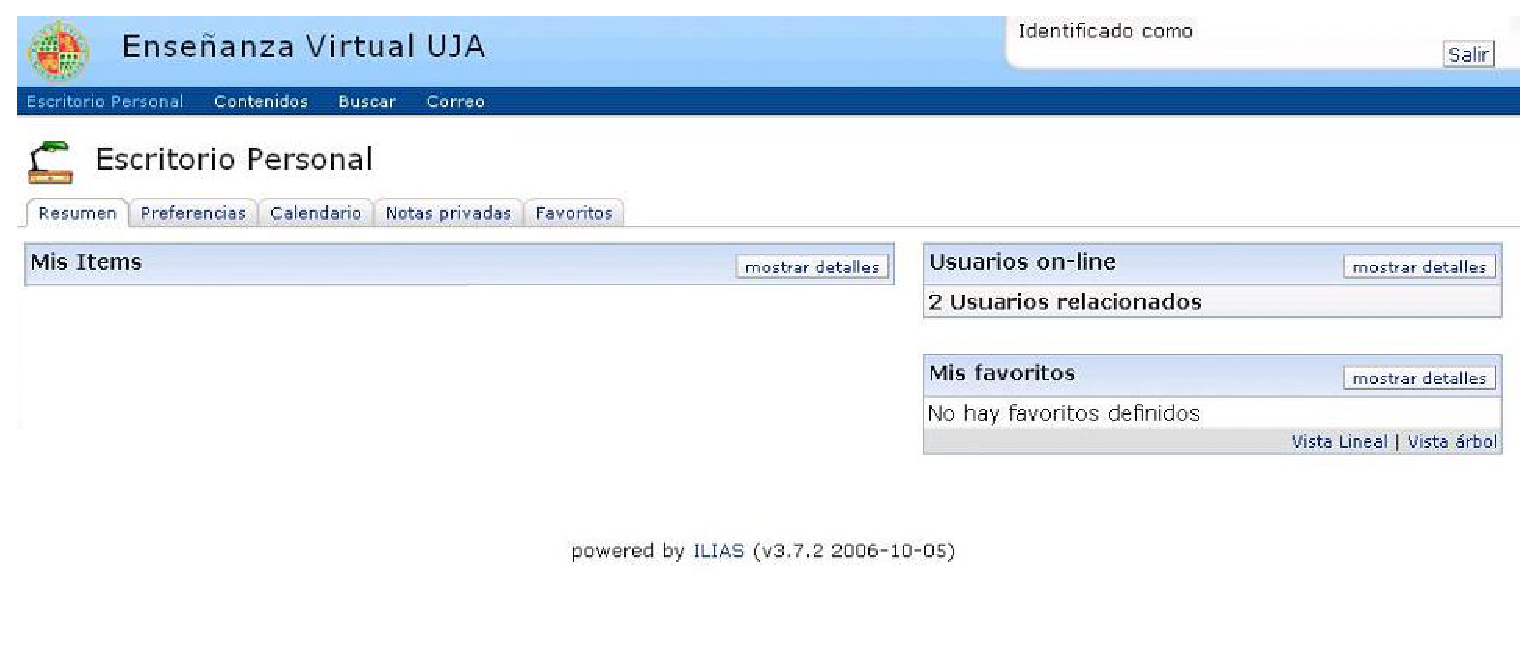
\includegraphics[width=\textwidth]{./img/c2-ilias.eps}
	\caption{Plataforma e-learning Ilias}
\end{figure}

\subsection{Requerimientos}

\begin{itemize}
	\item Servidor de aplicaciones: PHP 4.3.2. 
	\item Coste aproximado: Gratis.
	\item Base de datos: MySQL 4.0.14 o superior. Licencia: GNU GPL.
	\item Sistema operativo: Desarrollado con RedHat Linux 7.x/8.0 pero se puede usar sobre cualquier distribución Linux, Solaris o Unix.
	\item Lenguaje de programación: PHP. 
	\item Servidor web: Apache.
\end{itemize}

\subsection{Seguridad}

La seguridad en el sistema ILIAS se limita a la autenticación de los usuarios mediante un servidor externo LDAP o mediante el uso del protocolo RADIUS. Por otra parte, se permite la creación de distintos perfiles para mejorar el control de accesos a los recursos. Otro punto importante introducido en la última versión es el control de virus en la subida de ficheros.

\subsection{Soporte}

El soporte del sistema se limita a la información que contiene la web de la plataforma, \url{http://www.ilias.uni-koeln.de/ios/index-e.html}, en el apartado docs, que contiene documentos sobre instalación, desarrollo y migración entre distintas versiones de ILIAS. Además de estos documentos, en la misma web se encuentra un foro de discusión donde se pueden realizar consultas sobre la plataforma.

\subsection{Facilidad de uso}

ILIAS tiene una excelente facilidad de uso, permitiendo la inclusión de múltiples tipos de ficheros en los cursos, como pueden ser, módulos de aprendizaje ILIAS, test ILIAS, libros digitales, ficheros HTML, ficheros PDF, hojas de cálculo EXCEL, ficheros WORD, etc. Para la edición de los contenidos se integra un editor basado en XML con una interfaz XHTML con funciones de edición para texto, tablas, mapas, glosario, etc. Permite la integración de imágenes, applets, animaciones, video y audio. Por último decir que también permite el uso de hojas de estilos (CSS) y la reusabilidad de objetos mediante ILIAS VRI (Virtual Ressource Identifiers).

\subsection{Funciones}

La plataforma ILIAS posee distintas funciones de cacheado de páginas y la posibilidad de exportar información de manera estática para uso local. En su contra decir que no posee la función de replicado de bases de datos ni balanceo de carga.

\subsection{Administración}

La administración de la plataforma se limita a permitir o no permitir accesos a los contenidos por parte de los usuarios. Para ello jerarquiza los usuarios en función de perfiles o roles con diferentes niveles de acceso. Los perfiles de esta plataforma son los siguientes: profesor, estudiante, diseñador e invitado.

\subsection{Interoperatividad}

Como herramientas de interoperatividad la plataforma ILIAS posee foros de discusión que pueden ser introducidos en los cursos generados. Estos foros poseen las funciones normales de los mismos, editar mensajes, adjuntar ficheros, etc. Además de estos foros de discusión, ILIAS posee listas de correo tanto internas como externas que permiten la comunicación entre los usuarios de la plataforma. Por último, decir que posee un Chat para la comunicación en tiempo real de los usuarios.

\subsection{Aplicaciones soportadas}

ILIAS posee gran cantidad de aplicaciones que dan soporte a los cursos generados, como pueden ser Chats, foros, calendarios, estadísticas, etc. La plataforma ILIAS, además, posee gran cantidad de herramientas para fomentar el trabajo en grupo, permitiendo el intercambio de ficheros, la creación de contenidos de manera cooperativa, creación de foros para grupos, creación de calendarios de grupo y un organizador de tareas. En cuanto al tratamiento de los usuarios, ILIAS realiza su administración en función de cursos o bien en función de grupos (GroupWare).

\section{Proyecto Sakai}

\subsection{Introducción}

Plataforma desarrollada en conjunto por la Universidad de Mighigan, Universidad de Indiana, el MIT, Stanford y el consorcio uPortal con el objetivo de integrar y sincronizar su software educativo en una colección pre-integrada de herramientas de Open source para e-learning.

\begin{figure}[h]
	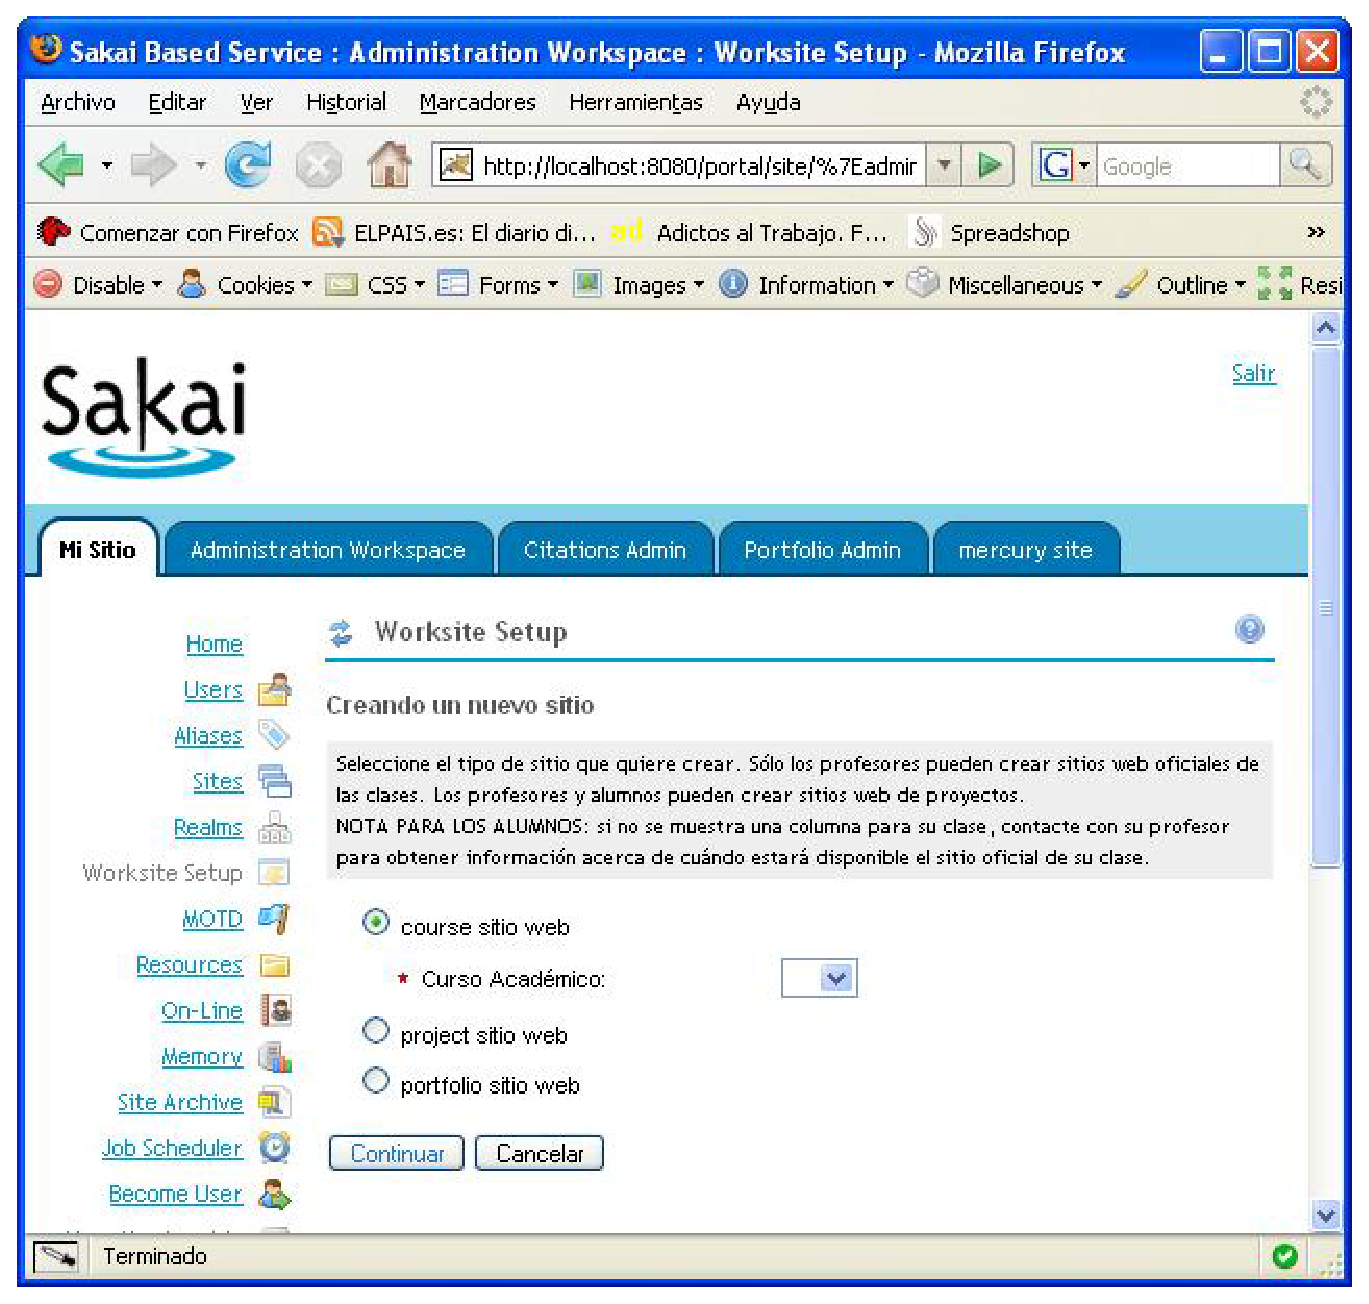
\includegraphics[width=\textwidth]{./img/c2-proyectosakai.eps}
	\caption{Plataforma e-learning Sakai}
\end{figure}

\subsection{Requerimientos}

\begin{itemize}
	\item Servidor de aplicaciones: J2EE.
	\item Coste aproximado: Gratuito o mínimo.
	\item Base de datos: MySQL u Oracle.
	\item Licencia: Open Source.
	\item Sistema operativo: Windows XP , Macintosh Mac Os, Linux o Solaris. 
	\item Lenguaje de programación: Java.
	\item Servidor web: TomCat.
\end{itemize}

\subsection{Seguridad}

En cuanto a la seguridad ofrecida por SAKAI\cite{sakai}, no se ofrecen datos técnicos en cuanto a la tecnología usada, simplemente se menciona que la seguridad es gestionada mediante Java y las tecnologías que contiene para esta función, permitiendo administración de características como autenticación. Un punto a favor de esta plataforma es que, al ser de carácter libre, se dispone del código fuente, por lo tanto en cualquier momento se pueden modificar los protocolos de seguridad y solventar problemas de seguridad del software.

\subsection{Soporte}

El soporte del sistema tiene dos apartados. Uno gratuito que se limita a la información que contiene la web de la plataforma \url{http://www.sakaiproject.org} que contiene documentos sobre instalación, desarrollo y migración entre distintas versiones de SAKAI. Por otro lado, tiene soporte comercial ofrecido por diferentes compañías que ofrecen hosting, instalación, migración, etc. Este soporte se ofrece con la versión comercial de la plataforma, la cual tiene un coste económico.

\subsection{Facilidad de uso}

En cuanto al uso de la plataforma SAKAI, decir que se permite la agregación de todo tipo de documentos de manera sencilla, como por ejemplo: ficheros HTML, ficheros PDF, hojas de cálculo EXCEL, ficheros WORD, etc. La interfaz de uso es una GUI (Graphical User Interface) basa en XML, mediante la cual se pueden gestionar todas las características del curso que se está creando.

\subsection{Funciones}

SAKAI posee como característica más importante la escalabilidad, puesto que posibilita el trabajo tanto con bases de datos de pequeño tamaño como de gran tamaño. Otras características importantes son que permite cacheado de la información y balanceo de carga, permitiendo así un mejor uso del sistema, disminuyendo la posibilidad de sobrecargas en el mismo.

\subsection{Administración}

La administración de los cursos en la plataforma SAKAI permite la creación de sitios individuales para los cursos realizados, la gestión de usuarios en cada uno de ellos así como la creación de subgrupos dentro de cada uno de los cursos. En cuanto a los contenidos de los cursos se permite la administración tanto de su contenido como del acceso al mismo.

\subsection{Interoperatividad}

Las herramientas para la interoperatividad ofrecidas por esta plataforma son foros de discusión, Chats en tiempo real, listas de correo, anuncios, calendarios, etc. De esta manera, se da soporte a la comunicación entre los usuarios de los cursos. Además de lo anteriormente mencionado, se permite la inclusión de información previa por parte del administrador del sistema o, incluso, por parte de cualquier usuario del sistema. La plataforma SAKAI ofrece soporte para el trabajo en grupo (Groupware), dando también soporte para el desarrollo e investigación online.

\subsection{Aplicaciones soportadas}

En cuanto a las aplicaciones soportadas por SAKAI decir que no tiene limite, puesto que funciona mediante servicios web. Por lo tanto cualquier aplicación puede ser adaptada e introducida dentro del portal como servicio web. Por otro lado, tenemos las APIs de programación de la plataforma mediante las cuales se pueden desarrollar nuevas aplicaciones para los cursos.

\section{Atutor}

\subsection{Introducción}

ATutor\cite{atutor} es un Sistema de Gestión de Contenido Educativo Basado en la Web, diseñado en la accesibilidad y la adaptabilidad. De esta manera, permite a los educadores desarrollar fácilmente contenido en línea en un ambiente de aprendizaje estructurado y adaptable. En cuanto a los estudiantes, permite navegar a través del contenido de diferentes maneras, de acuerdo a su estilo o método preferido de aprendizaje en línea. ATutor está disponible de manera gratuita para uso no comercial bajo GNU GLP, permitiendo la distribución y modificación del código fuente provisto siempre y cuando el derecho de autor y las líneas de crédito no sean alteradas.

\begin{figure}[h]
	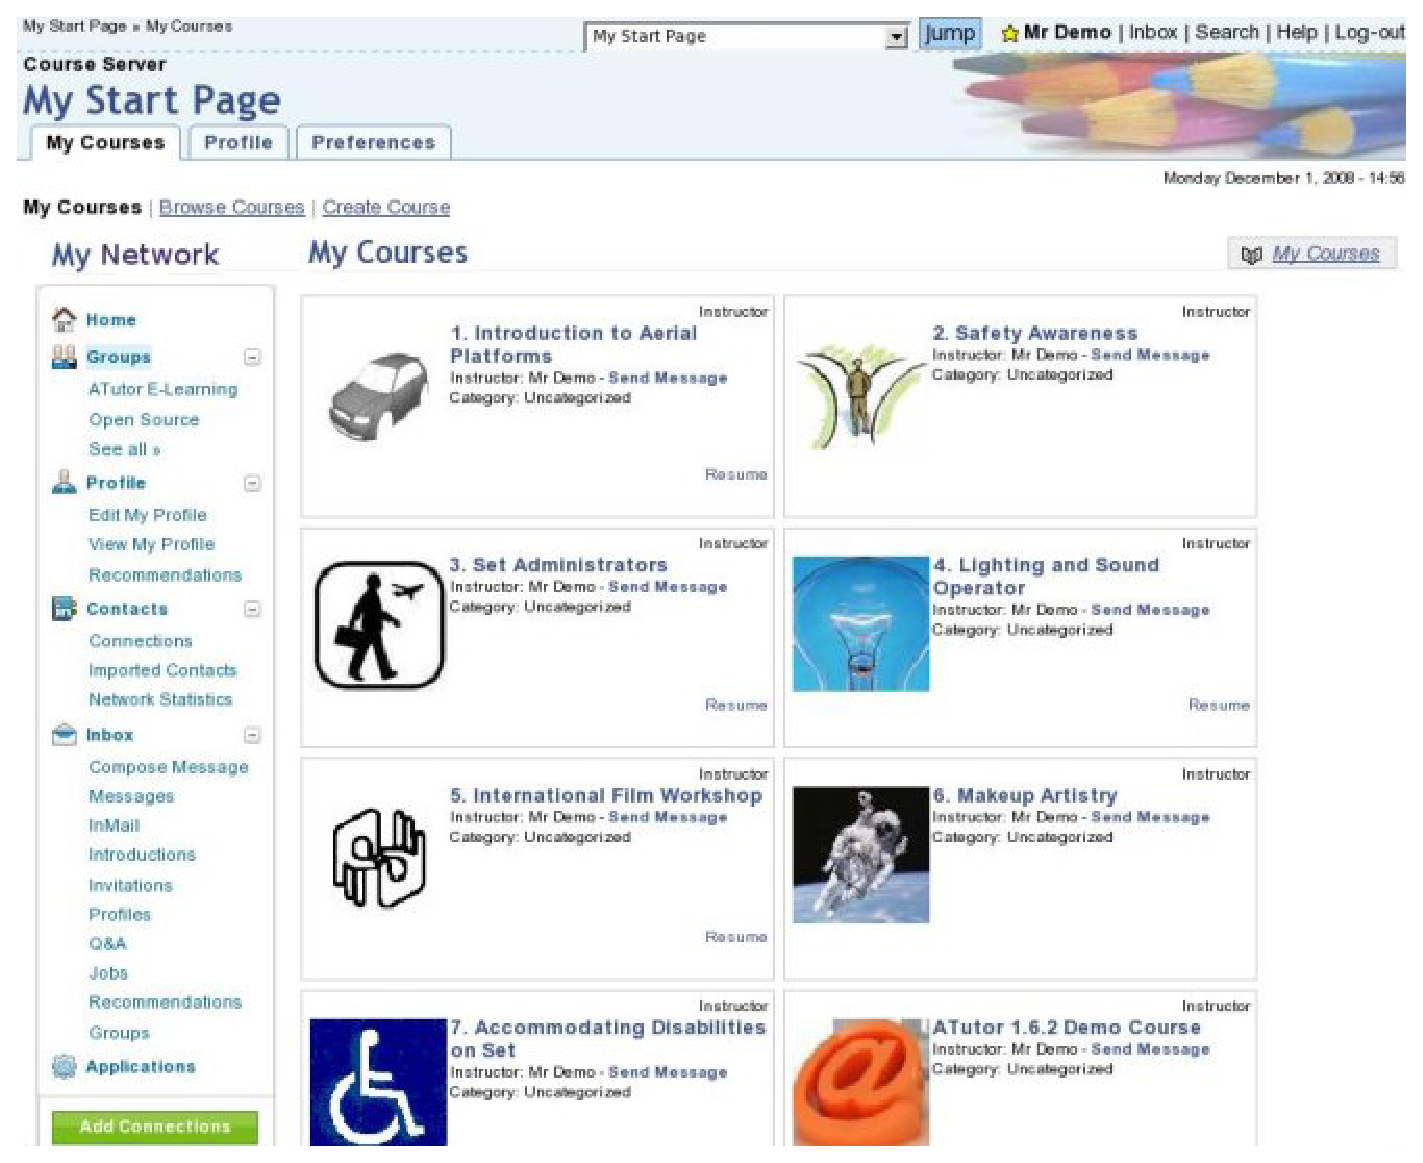
\includegraphics[width=\textwidth]{./img/c2-atutor.eps}
	\caption{Plataforma e-learning ATutor}
\end{figure}

\subsection{Requerimientos}

\begin{itemize}
	\item Servidor de aplicación: PHP 4.1.2+. 
	\item Coste aproximado: Gratis.
	\item Base de datos: MySQL.
	\item Licencia: GNU GPL.
	\item Sistema operativo: Cualquiera. 
	\item Lenguaje de programación: PHP. 
	\item Servidor Web: Apache 1.3.
\end{itemize}

\subsection{Soporte}

En cuanto a lo que se refiere al soporte, Atutor no tiene ningún manual comercial en el mercado aunque sí proporciona una ayuda on-line, un foro público, una lista de correo y manuales para su utilización.

\subsection{Facilidad de uso}

Es un LMS (Learning Management System) con gran soporte para realizar cursos y caracterizado por poseer funciones de colaboración. Además, está diseñado para una fácil accesibilidad, para su uso en varias lenguas y para el cumplimiento de especificaciones e-learning. Posee una buena ayuda on-line y un tutorial para nuevos usuarios. Además se sustenta en los mejores recursos open source, Apache, PHP y MySQL.

\subsection{Funciones}

Esta plataforma posee varias funciones siempre orientadas a mejorar la accesibilidad y facilitar el uso. En cuanto a aspectos relacionados con este apartado encontramos que posee navegación adaptativa, permitiendo a cada usuario configurar los contenidos de sus cursos. Otra función importante es la posibilidad de exportación de los contenidos de la base de datos.

\subsection{Administración}

El apartado de administración del aTutor posee menos características con respecto a los CMS vistos, esto es debido a que .aTutor.es una plataforma orientada al aprendizaje (LMS). Aunque también hay que decir que la funcionalidad incluida en el apartado de administración es la idónea para el correcto funcionamiento de los cursos desarrollados.

\subsection{Interoperatividad}

En este apartado aTutor supera a las plataformas anteriores permitiendo la comunicación mediante las aplicaciones vistas en los anteriores CMS, como son Chats, foros, etc. Pero además posee un módulo de trabajo colaborativo que está integrado dentro de la plataforma (aCollab).

\subsection{Aplicaciones soportadas}

aTutor posee una serie de aplicaciones, cada una de ellas con una funcionalidad clara definida:

\begin{itemize}
	\item aCollab: aplicación que permite el trabajo colaborativo así como la creación de grupos dentro de los cursos.
	\item aChat: esta aplicación como se puede observar posee un nombre bastante identificativo de su función, es decir, permite crear Chats dentro de los cursos.
	\item aComm: esta aplicación permite el uso de una pizarra, además de permitir la comunicación entre usuarios.
	\item aTalker: aplicación que realiza las funciones de "specher", es decir, lee un texto escrito dentro del curso.
\end{itemize}

\section{eGroupWare}

\subsection{Introducción}

eGroupware\cite{egroupware} es una sistema de trabajo en grupo vía web, de código abierto. Está escrita en PHP utilizando bases de datos, tales como PostgreSQL o MySQL. Incluye un calendario, una libreta de direcciones, un gestor de contactos, un cliente de correo electrónico IMAP, un InfoLog, funciones de CRM (Customer Relationship Management), un gestor de proyectos, un gestor de recursos, un gestor de ficheros, una plantilla de tiempos, un wiki, una base de conocimiento y un motor de flujos de trabajo.

\begin{figure}[h]
	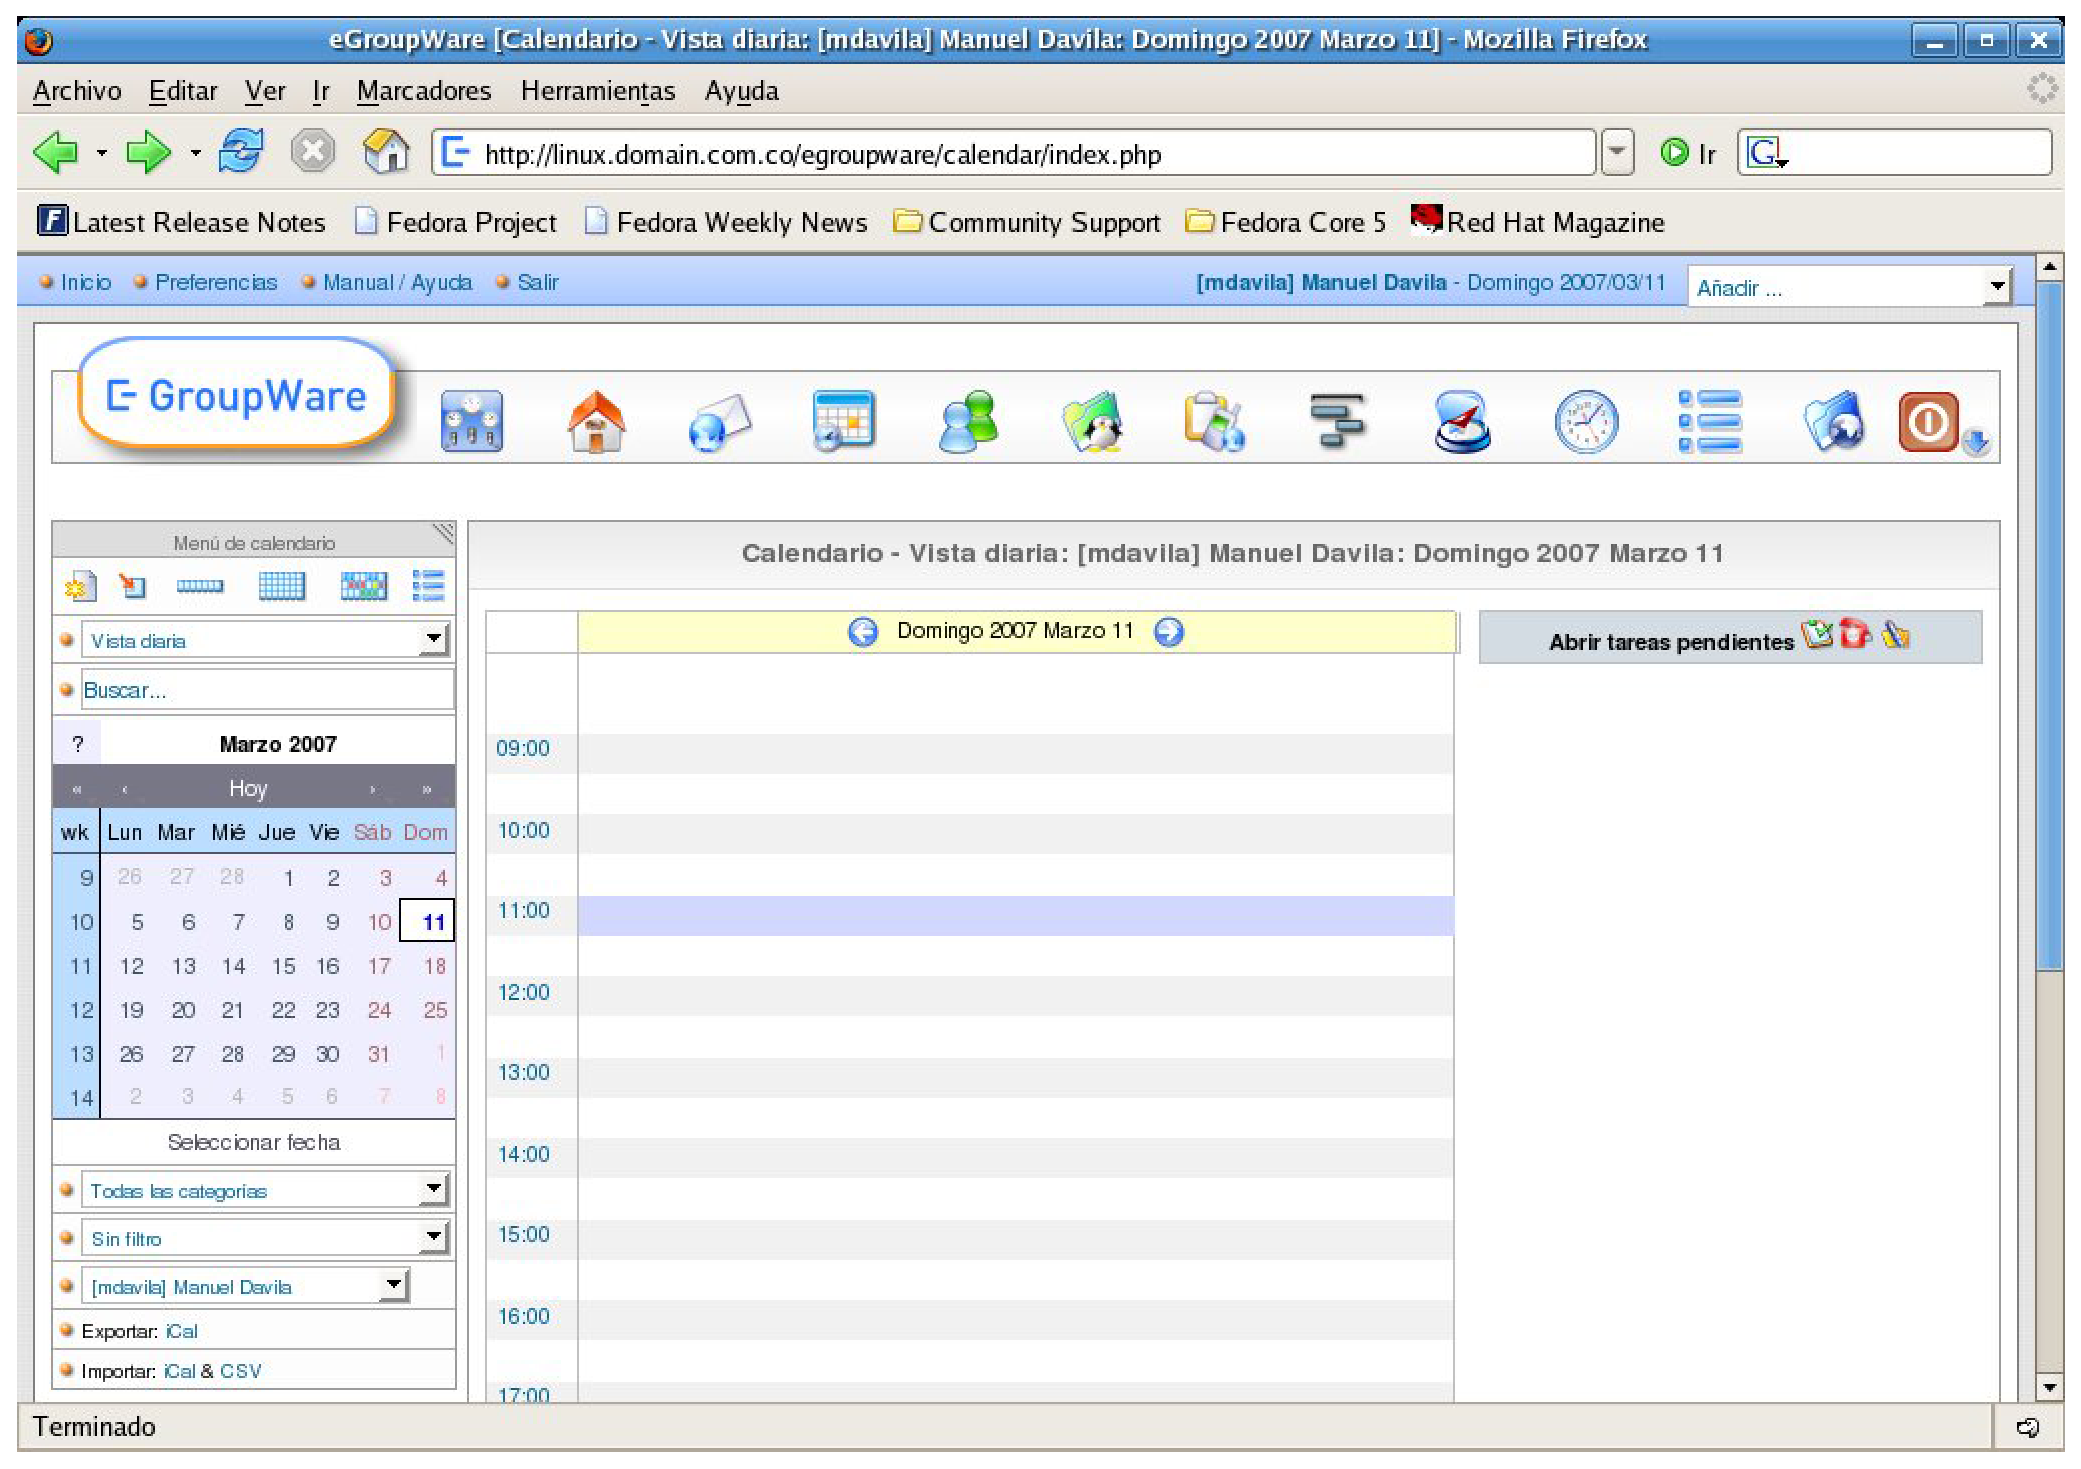
\includegraphics[width=\textwidth]{./img/c2-egroupware.eps}
	\caption{Plataforma e-learning EGroupWare}
\end{figure}

\subsection{Requerimientos}

\begin{itemize}
	\item Servidor de aplicación: PHP 4.3+ como mínimo, aunque se recomienda PHP 5.1+ pues se puede requerir alguna funcionalidad de esta versión como son las notificaciones y las utilidades de exportar e importar.
	\item Coste aproximado: Gratis.
	\item Base de datos: MySQL 4.1+, aunque se recomienda la versión 5.0+ (la mayor parte del trabajo funciona correctamente en la versión 4.0 pero módulos como la lista de precios en el gestor de proyectos así como la base de conocimiento no. Otra opción es utilizar Postgres 8.0+.
	\item Licencia: GNU GPL.
	\item Sistema operativo: Cualquiera.
	\item Lenguaje de programación: PHP.
	\item Servidor Web: Cualquiera que soporte PHP. Entre los más importantes se encuentran:
	\begin{itemize}
		\item Apache version 1.33+ 
		\item IIS
		\item Roxen
	\end{itemize}
\end{itemize}

\subsection{Seguridad}

La seguridad en el sistema eGroupWare está bastante definida y ofrece una serie de servicios, de entre los que destaca:

\begin{itemize}
	\item Seguridad básica en el servidor. Se pueden elegir muchas posibilidades para tener seguridad en el servidor:
	\begin{itemize}
		\item La medida de seguridad más importante que se puede hacer es mantener la instalación actualizada. Para estar informado de las nuevas actualizaciones existe una lista de correo a la que cualquier usuario del sistema puede suscribirse.
		\item Comprobar los servicios que se ejecutan y puertos abiertos.
		\item Desinstalar programas que no se necesitan en el servidor.
		\item Comprobación local de existencia de un rootkit.
		\item Administración de un servidor seguro, realizando conexiones en modo seguro, trabajando con pares de claves SSH, etc.
		\item Instalar software para monitorizar los registros del sistema.
		\item Entorno de detección de intrusos.
		\item Seguridad de los servicios en demonios.
		\item Cortafuegos.
	\end{itemize}
	\item Seguridad en aplicaciones web. Con un software de seguridad en aplicaciones, se pueden ejecutar de forma segura las aplicaciones basadas en web, como eGroupWare, desde ejecuciones SQL, Cross Side Scripting y otros ataques. Hay varias aplicaciones en el mercado Apache e IIS.
	\item Optimización y seguridad en Apache. Para la seguridad del servidor web, se deben desactivar todos los módulos innecesarios así como activar sólo los que se necesite para ejecutar el servidor web. Ejecutarlo con menos módulos, también mejora el rendimiento.
	\item Seguridad de la instalación PHP.
	\item Crear un certificado para el servidor web. Para proteger su privacidad, si se conecta a una instalación eGroupWare, se puede usar un certificado en el servidor. Con un certificado, se puede conectar al servidor web con una conexión cifrada (https en vez de http). Sin una conexión https, otras personas pueden usar un Sniffer para averiguar la contraseña, u otra información.
\end{itemize}

\subsection{Soporte}

En cuanto al soporte, eGroupWare posee un sitio web oficial muy completo en el que existe una amplia variedad de manuales así como un foro público, una lista de correo, ayuda on-line, etc.

Además, desde la misma web de eGroupWare se puede también tener comunicación directa con desarrolladores experimentados, concertar citas o entrevistas, etc.

\subsection{Facilidad de uso}

El sistema eGroupWare posee una interfaz muy intuitiva y fácil de utilizar. De esta manera, el menú principal proporciona rápidos enlaces hacia la página personal del usuario, hacia el módulo general de preferencias personales, hacia información relativa a un módulo específico así como para funciones de cierre de sesión.

\subsection{Funciones}

Como se ha comentado anteriormente, el sistema eGroupWare ofrece una funcionalidad muy extensa y variada. Entre estas funciones destacan:

\begin{itemize}
	\item Calendario.
	\item Libreta de direcciones.
	\item Gestor de contactos.
	\item Cliente de correo electrónico IMAP. InfoLog.
	\item Funciones de CRM.
	\item Gestor de proyectos.
	\item Gestor de recursos.
	\item Gestor de ficheros.
	\item Plantilla de tiempos.
	\item Una wiki.
	\item Una base de Conocimiento.
	\item Un motor de flujos de trabajo.
\end{itemize}

\subsection{Administración}

En lo que se refiere a administración, en eGroupWare se permitirá administrar tanto las cuentas de usuario como los grupos de usuarios.

Hay que tener en cuenta que la administración de grupos de usuarios es más compleja que la de cuentas de usuario, pues estas últimas únicamente necesitan su creación, su posible modificación y su cancelación. Sin embargo, la administración de grupos requiere otras operaciones.

Separar los usuarios en grupos proporciona una manera de controlar qué modulos están disponibles para cada grupo (Correo, calendario, administrador de ficheros). También proporciona al administrador una forma de controlar qué grupos tienen acceso a otros grupos o información de usuarios. Al igual que una empresa tiene distintos departamentos, también los tiene eGroupWare. Por ejemplo, el departamento de compras puede no necesitar el módulo del Administrador de ficheros, y el departamento legal sí lo necesita para compartir documentos entre miembros o grupos del departamento. Al configurar el grupo del departamento legal, se marcaría el módulo del administrador de ficheros. Al configurar el grupo de compras, se asegura no marcar el módulo del administrador de ficheros.

eGroupWare permite poder tener todos los módulos disponibles para todos los grupos, pero el administrador controlaría qué grupo tiene acceso a la información de otro grupo mediante ACLs (Listas de control de accesso).

Es necesario realizar una preparación y una planificación para implantar eGroupWare en una empresa. Como todos los proyectos, en esta parte es donde se dedica la mayor parte del tiempo. Organizar los grupos y planear los privilegios de acceso. Preguntar quién necesita qué y por qué es un comienzo.

\subsection{Interoperatividad}

Como herramientas de interoperatividad, la plataforma eGroupWare posee foros de discusión y wikis. Estos foros poseen las funciones normales de los mismos, edición de mensajes, adjuntar ficheros, etc. En cuanto a los wikis ofrecen una herramienta para la construcción de conocimiento para la comunidad. Cada página en un Wiki es parecida a una página web excepto en que todo el mundo puede editarla. Esto hace a los Wikis una herramienta ideal para capturar conocimiento.

Ademas de todo esto posee funciones de CRM (Customer Relationship Management), un gestor de proyectos (a partir de diagramas de Gantt), un gestor de recursos, etc.

\subsection{Aplicaciones soportadas}

El sistema eGroupWare está formado por un conjunto de aplicaciones individuales e instalables. Todas estas aplicaciones tienen como objetivo dar solución a un problema relativo al trabajo colaborativo. Las aplicaciones más importantes dentro de este sistema pueden ser:

\begin{itemize}
	\item Calendario.
	\item Libro de direcciones. Es una aplicación para la gestión de clientes u otra relativa a la información de contactos, y enlazarla con otras aplicaciones egroupware. Se pueden importar y exportar contactos en formatos como LDIF, CVS o VCard y administrarlos por SQL o LDAP.
	\item FelaMiMail. Es una aplicación e-mail para el trabajo colaborativo que se puede enlazar con otras aplicaciones como es el caso del libro de direcciones.
	\item InfoLog
\end{itemize}

\section{Comparativa de la plataforma para la gestión docente}

Lo primero que debe tenerse en cuenta al tomar dicha decisión es que la plataforma debe ser gratuita y que tenga los requisitos software para favorecer la minimización de costes en el desarrollo del proyecto.

De esta manera y fijándonos en el coste de la licencia, se va a desechar el uso de WebCT, puesto que se trata de una plataforma de pago.

En este punto nos encontramos ante la decisión de usar una de las siguientes plataformas: ATutor, Moodle, Ilias y eGroupWare. La primera que descartaríamos, de entre estas cuatro, es eGroupWare pues aunque permite trabajo colaborativo no está destinado al aprendizaje. Por tanto nos quedarían sólo las tres primeras como opciones candidatas. Para la elección de una de ellas, realizaremos una comparativa detallada de características y funcionalidades de las tres, analizando los siguientes aspectos:

\begin{itemize}
	\item Acceso.
	\item Seguimiento.
	\item Soporte del software.
	\item Funciones a disposición del alumno. Administración.
	\item Facilidad de uso.
	\item Otros.
\end{itemize}

\newpage
\subsection{Acceso}

\begin{table}[h]
\centering
\begin{tabular}{ | p{0.15\textwidth} | p{0.24\textwidth} | p{0.24\textwidth} | p{0.24\textwidth} | }
	\hline
	  & \textbf{ATutor} & \textbf{Ilias} & \textbf{Moodle} \\
	\hline 
	Autenticación  & 
	Pide el usuario y clave, además de tener la opción de login automático. & 
	Pide usuario y clave utilizando el protocolo LDAP. Además el administrador puede crear grupos con distintos privilegios.  & 
	Pide usuario y clave utilizando el protocolo LDAP. Además permite el registro mediante la confirmación de clave por e-mail.  \\
	\hline
	Invitados &
	Permite el acceso a todos los contenidos de los cursos públicos. &
	Solo permite el acceso a la sección de registro on-line. &
	Permite el acceso a todos los contenidos de los cursos públicos. \\
	\hline
	Acceso al curso &
	Se pueden crear distintos tipos de cursos según sus privilegios de acceso: público (puede entrar cualquier usuario), protegido (sólo se permite el acceso de los alumnos registrados en el curso) y privado (solo se permite el acceso de aquellos alumnos registrados y autorizados por el profesor del curso). &
	Sólo se permite el acceso de los usuario registrados. &
	Se pueden crear cursos públicos y privados. Los públicos permiten el acceso de usuarios registrados y de invitados. Los privados sólo pueden ser vistos por los usuarios registrados, es decir, alumnos confirmados por los profesores. \\
	\hline
\end{tabular}
\caption{Comparativa de Acceso}
\end{table}

\newpage
\subsection{Seguimiento}

\begin{table}[h]
\centering
\begin{tabular}{ | p{0.15\textwidth} | p{0.24\textwidth} | p{0.24\textwidth} | p{0.24\textwidth} | }
	\hline
	  & \textbf{ATutor} & \textbf{Ilias} & \textbf{Moodle} \\
	\hline 
	Seguimiento en el acceso  & 
	El seguimiento en un curso debe estar autorizado por el administrador mediante una opción de configuración. A partir de este momento el seguimiento del usuario que ha entrado en el curso es completo, pudiendo ver todas las actividades que realiza, etc. Además, tiene la opción de ver un histograma y exportar a un fichero Excel. & 
	El administrador decide en cada curso cuáles son los parámetros del seguimiento: acceso, foros, etc. El profesor puede ver las estadísticas de su propio curso.  & 
	Tanto los profesores como el administrador pueden ver el seguimiento del alumno. Los profesores tienen acceso sólo a los cursos de los que son profesores. El seguimiento es completo sobre todas las actividades que realiza el alumno y se puede visualizar con respecto a cada actividad o dato preciso.  \\
	\hline
\end{tabular}
\caption{Comparativa de Seguimiento}
\end{table}

\newpage
\subsection{Soporte del Software}

\begin{table}[h]
\centering
\begin{tabular}{ | p{0.18\textwidth} | p{0.24\textwidth} | p{0.24\textwidth} | p{0.24\textwidth} | }
	\hline
	  & \textbf{ATutor} & \textbf{Ilias} & \textbf{Moodle} \\
	\hline 
	Documentación  & 
	La documentación oficial de Atutor es completa y fácil de usar. Existen cursos sobre Atutor pero hay que estar registrados. & 
	La documentación oficial no es muy descriptiva y específica, sólo ofrece una visión global. Hay documentación no oficial que está más completa (en inglés).  & 
	A parte de cursos de Moodle en la página oficial, también existe documentación completa y detallada tanto oficial como no oficial para el administrador, profesores y usuarios.  \\
	\hline
	Soporte técnico  & 
	Existen foros en la comunidad de Atutor de soporte. & 
	Existen foros en la comunidad de Atutor de soporte. & 
	Igual que los anteriores, además posee Chats que, a horas específicas, están disponibles para cualquier duda.  \\
	\hline
\end{tabular}
\caption{Comparativa de Soporte del Software}
\end{table}

\subsection{Funciones a disposición del alumno}
\begin{center}
\begin{longtable}{| p{0.18\textwidth} | p{0.24\textwidth} | p{0.24\textwidth} | p{0.24\textwidth} |}
	\hline
	  & \textbf{ATutor} & \textbf{Ilias} & \textbf{Moodle} \\
	\hline 
	\endfirsthead
	\hline
	  & \textbf{ATutor} & \textbf{Ilias} & \textbf{Moodle} \\
	\hline 
	\endhead
	
	% aquí añadimos el fondo de todas las hojas, excepto de la última.
	\multicolumn{4}{c}{Sigue en la página siguiente.}
	\endfoot

	% aquí añadimos el fondo de la última hoja.
	\endlastfoot
	
	Foro  & 
	Posee foros típicos por medio de hilos. Puede ser público o privado dependiendo del curso. & 
	Los Foros vienen dados por preguntas. La persona que crea el curso decide en qué cursos lo quiere crear. Se pueden crear cursos para grupos.  & 
	Foro basado en hilos. También usado para las noticias y novedades. Configurable dependiendo de qué usuarios lo utilizarán si profesores o alumnos. También se pueden evaluar.  \\
	\hline
	Descarga de archivos  & 
	Cada profesor pone a disposición de los alumnos los archivos. & 
	Tanto el profesor como un grupo puede cargar y poner una dirección URL para bajarse el archivo. No se carga al servidor. & 
	Tanto los profesores como los alumnos pueden dejar archivos en foros o en las actividades donde puedan y los profesores lo permitan.  \\
	\hline
	Lista de correo & 
	Posee mensajería interna entre dos personas. Sin embargo, no se puede enviar de uno a varios, aunque sí se puede a todos los inscritos a un curso. & 
	El administrador decide el acceso a los correos. Se pueden mandar tanto correos como mensajería privada a una o varias personas y a un grupo. & 
	Se pueden enviar tanto correos, como mensajería privada entre dos personas. \\
	\hline
	Test on line & 
	Los profesores pueden crear tests on-line y asignarle un tiempo de vida. Los alumnos no pueden saber las respuestas cuando terminan el test.& 
	Los profesores pueden crear tests on-line y asignarle un tiempo de respuesta. Ofrece la posibilidad de linkar un documento que contenga la respuesta. Una vez terminado el test indica las respuestas correctas y cuales son las que ha puesto el estudiante. & 
	Los profesores pueden crear tests on-line y asignarle un tiempo de vida. Los alumnos sí pueden saber las respuestas cuando terminan el test. También permiten bajar un link con un documento donde están las respuestas. \\
	\hline
	Chat & 
	Posee un Chat basado en PHP en el que se puede entrar una vez matriculado en el curso. & 
	Posee Chat mediante la instalación de un módulo. & 
	Posee Chat, siempre que el profesor lo haya creado en un curso. \\
	\hline
	Otros & 
	Posee diferentes paquetes como pueden ser speaker, Chat, grupos colaborativos, pizarrra, etc, pero pocos traducidas al español. & 
	Posee Chat y otras actividades como módulos complementarios. & 
	Módulos como el de reunión, libro, flash, wikis, encuestas, talleres, tareas, etc. \\
	\hline

\caption{Comparativa de Funciones a disposición del alumno}
\end{longtable}
\end{center}

\subsection{Administración}

\begin{center}
\begin{longtable}{| p{0.18\textwidth} | p{0.24\textwidth} | p{0.24\textwidth} | p{0.24\textwidth} |}
	\hline
	  & \textbf{ATutor} & \textbf{Ilias} & \textbf{Moodle} \\
	\hline 
	\endfirsthead
	\hline
	  & \textbf{ATutor} & \textbf{Ilias} & \textbf{Moodle} \\
	\hline 
	\endhead
	
	% aquí añadimos el fondo de todas las hojas, excepto de la última.
	\multicolumn{4}{c}{Sigue en la página siguiente.}
	\endfoot

	% aquí añadimos el fondo de la última hoja.
	\endlastfoot
	Gestión y mantenimiento del LCMS  & 
	Apenas se accede al sistema como administrador se visualizan las opciones de cambio de rol y las características generales del sitio. El administrador tiene la posibilidad de editar sus datos, así como su rol, modificar los datos de un curso, el lenguaje, etc. La complejidad de esta labor depende del tamaño del portal. & 
	El administrador tiene la responsabilidad de todo y además puede hacer todo lo que haga un docente. Puede gestionar cuentas, módulos de Ilias, los foros, el sistema (aspecto, lenguaje, base de datos, etc.), el seguimiento, etc.  & 
	Parecida a la de Atutor, puede gestionar todas las cuentas, todos los cursos, las variables del sistema, también puede cambiar de rol. La complejidad de esta labor depende del tamaño del portal.  \\
	\hline
\caption{Comparativa de Administración}
\end{longtable}
\end{center}

\newpage
\subsection{Facilidad de uso}
\begin{center}
\begin{longtable}{| p{0.18\textwidth} | p{0.24\textwidth} | p{0.24\textwidth} | p{0.24\textwidth} |}
	\hline
	  & \textbf{ATutor} & \textbf{Ilias} & \textbf{Moodle} \\
	\hline 
	\endfirsthead
	\hline
	  & \textbf{ATutor} & \textbf{Ilias} & \textbf{Moodle} \\
	\hline 
	\endhead
	
	% aquí añadimos el fondo de todas las hojas, excepto de la última.
	\multicolumn{4}{c}{Sigue en la página siguiente.}
	\endfoot

	% aquí añadimos el fondo de la última hoja.
	\endlastfoot
	
	Alumnos  & 
	En general en todas la tareas comunes de los alumnos como son: crear una cuenta, acceder a un curso, hacer una actividad, particpar en un foro o chat, mandar un mensaje privado o resolver algún problema con la ayuda de otros alumnos, se hace sin ningún problema. & 
	En general en todas la tareas comunes de los alumnos como son, crear una cuenta, acceder a un curso, hacer una actividad, particpar en un foro o chat, mandar un mensaje privado o resolver algún problema con la ayuda de otros alumnos se hace sin ningún problema. & 
	En general en todas las tareas comunes de los alumnos como son, crear una cuenta, acceder a un curso, hacer una actividad, particpar en un foro o chat, mandar un mensaje privado o resolver algún problema con la ayuda de otros alumnos se hace sin ningún problema. Moodle posee además una ayuda en cada contenido.  \\
	\hline
	Profesores  & 
	Para las funciones de los profesores como son crear una cuenta, un curso, configurar éste, agregar actividades, etc, es amigable y fácil de usar. Posee un interfaz diferente al de los alumnos con lo que queda un poco engorroso. & 
	Para las funciones de los profesores como son crear una cuenta, un curso, configurar éste, agregar actividades, etc, es amigable y no tiene mucha dificultad. & 
	Para las funciones de los profesores como son crear una cuenta, un curso, configurar éste, agregar actividades etc. es amigable y fácil de usar, aunque pierde un poco de privilegios con respecto a Atutor, como puede ser a la hora de modificar el interfaz de la página.  \\
	\hline
	Administradores & 
	Las funciones de administración en Atutor no tienen una complejidad mayor que las demás. & 
	Complejidad similar a la de Atutor. & 
	Los tres están en la misma línea, aunque Moodle mantiene el mismo interfaz independientemente del usuario. \\
	\hline
\caption{Comparativa de Facilidad de uso}
\end{longtable}
\end{center}

\subsection{Otros}
\begin{center}
\begin{longtable}{| p{0.18\textwidth} | p{0.24\textwidth} | p{0.24\textwidth} | p{0.24\textwidth} |}
	\hline
	  & \textbf{ATutor} & \textbf{Ilias} & \textbf{Moodle} \\
	\hline 
	\endfirsthead
	\hline
	  & \textbf{ATutor} & \textbf{Ilias} & \textbf{Moodle} \\
	\hline 
	\endhead
	
	% aquí añadimos el fondo de todas las hojas, excepto de la última.
	\multicolumn{4}{c}{Sigue en la página siguiente.}
	\endfoot

	% aquí añadimos el fondo de la última hoja.
	\endlastfoot
	
	Idioma  & 
	Posee diferentes paquetes de distintas lenguas. En la versión analizada tenemos 8 lenguas, pero en desarrollo hay muchas más. & 
	El castellano está disponible pero con algunas deficiencias. & 
	Posee 34 lenguas, entre ellas el castellano, y se pueden especificar en cada curso.  \\
	\hline
	Soporte Multiplataforma  & 
	Soporta servidores Windows, Linux, y Unix. & 
	Soporta Linux y Solaris por igual. & 
	Soporta servidores Windows, Linux y Unix.  \\
	\hline
	Experiencia instalada & 
	Posee una gran comunidad y está numerosamente difundida en todo el mundo. La comunidad española no es muy grande. & 
	Poco difundido y la comunidad es prácticamente alemana. & 
	Posee una gran comunidad en castellano, además de su gran difusión, mucho mayor que las dos anteriores. \\
	\hline
	Posibilidad de la importación de paquetes y módulos & 
	Atutor puede importar cursos IMS. Una de sus puntos flacos es que no puede incorporar módulos como lo hace Moodle, sino que posee diferentes plataformas que se unen entre sí como son ACollab o AChat y que poseen interfaz diferente. & 
	Ilias puede importar cursos IMS, también tiene la posibilidad de importar algunos módulos. & 
	Puede importar cualquier paquete SCORM y próximamente podrá exportar e importar IMS. En lo que respecta a los módulos posee una gran extendibilidad en este sentido ya que tiene la posibilidad de instalar y desinstalar estos módulos que están en continúo desarrollo. \\
	\hline
\caption{Comparativa de otras características}
\end{longtable}
\end{center}

\section{Elección de la plataforma para la gestión docente}

Después de la comparación de todas estas características, la primera descartada sería Ilias debido a su pobre comunidad española y su insuficiente documentación y funcionalidad, además de su poca difusión.

Después de descartar Ilias, la elección estaría entre Moodle y Atutor. Aunque parezca una elección difícil, esto no es así. La elección sería Moodle fundamentalmente por las siguientes características:

\begin{itemize}
	\item Moodle posee una filosofía construccionista porque se centra en actividades interactivas del estudiante mientras que Atutor era fundamentalmente un entorno para "colgar apuntes" que con las nuevas versiones ha mejorado mucho, pero que, sin embargo, sigue sustentándose en una filosofía que afronta los cursos separando las actividades por tipo, es decir, están los foros por un lado, los exámenes por otro, los Chats por otro, etc. Esto en Moodle no es así pudiendo seguir una temática o un tiempo dependiendo de la configuración del curso aunque todo esto no es obligatorio.
	\item Moodle es modular. El profesor puede agregar o quitar actividades a su curso. A su vez, la plataforma también funciona de la misma manera pudiéndose desarrollar nuevos módulos y ser instalados. Atutor es monolítico, pues el profesor no tiene el diseño del aprendizaje en sus manos.
	\item Aunque ya ha sido evaluado en las tablas anteriores, la facilidad de uso en Moodle puede ser menos dificultosa que en Atutor debido a que éste cambia el interfaz dependiendo del usuario.
	\item La comunidad en castellano es muchísimo más superior la que tiene moodle que aTutor sin duda alguna, y el respaldo de la comunidad hace tener un número superior de foros que hacen que el desarrollo y la expansión de Moodle sea superior, sobre todo aquí en España.
\end{itemize}

Por supuesto, el hecho de elegir Moodle no es todo ventajas. También Atutor tiene algunas ventajas sobre Moodle como son:

\begin{itemize}
	\item La posibilidad de integrar IMS, que sin duda es el futuro de los estándares e-learning después de que SCORM esté siendo desechado. El equipo de Moodle trabaja sobre ello y dentro de poco estará operativo en forma de módulo.
\end{itemize}
